\section{Evaluation}
\label{sec:resul}

\subsection{Goals \& Workshop}
\par The purpose of the evaluation is to assess two things: how the children like the prototype in terms of enjoyment and satisfaction, i.e., whether they like the concept, have fun playing and want to play more; And the usability, whether the virtual and "real life" components of the game - interface and challenges - are adequate, and work well with each other, and individually.
\par To evaluate this, a workshop was conducted with children from a middle school in Austria. It consisted in two classes of children aged 10-12 years old, each class split in groups of 8 children. This was not always possible, so if needed one of us would fill in the role of the missing player. Each group had a session where they played as 4 different pairs - 4 play as Simon and the other 4 play Max - as if they were part of 4 different classes.  To decide who played as Simon and who played as Max, the children were seated in two rows of four: those in front would play as Max and those in the back play as Simon.
The markers were spread around the room before the workshop. Each session for a group took about 30 minutes, 5 for an introduction, 15 for the actual gameplay, and the remaining 10 to fill a quantitative questionnaire and have a little group discussion with some qualitative questions.
\par As the workshop was evaluating 4 pairs of players playing at the same time, new markers had to be created to accomodate that all those players. As Vuforia uses a grayscale image to recognize the pattern, new markers were devised with the same sketch but a different color, and a letter in the corner with the pair that belonged to (pair L,I,N, or A). However, Vuforia didn't properly distinguish the markers with the letters, so they become more indicative for the players than functional, as they could still scan a marker that "belonged" to another pair.

\subsection{Quantitative and Qualitative Instruments}

\par To evaluate the enjoyment/satisfaction and usability a quantitative questionnaire was constructed based on three scales: GSUS, an adapted version of SUS - System Usability Scale for game context \cite{molnar_kostkova_2014}, the Enjoyment subscale of GUESS - Game User Experience Satisfaction Scale \cite{phan_keebler_chaparro_2016} and the Interest/Enjoyment subscale of IMI - Intrinsic Motivation Inventory \cite{wilde_et_al_2009}. This questionnaire grouped some questions that were transversal to all three, and omitted others because it would take to long for the children to answer all the questions, plus some would not be suited for the children to answer, like the Usefulness subscale of IMI and GUESS. \par The answers were provided in a 5-point Likert scale with "thumbs up and down" images: "thumbs up" if they agreed with the statement, "thumbs down" if they disagreed. Also collected was their age, gender and class.

\par The focus interview followed a guide (based on the one from M Steiner et al. 2015)\cite{steiner_at_al_2015} with qualitative questions, also regarding enjoyment and usability, about their impression of the game and what they did and did not like in general, and two specific game components: the gameplay and the interface.

\subsection{Results}

\par These results were obtained from a population of 31 subjects - 13 males and 18 females, 9 being ten year-olds, 21 eleven year-olds and 1 thirteen year old - split in two classes: class 1A with 22 subjects - 10 males and 12 females - and class 1C with 9 subjects - 3 males and 6 females. 

\subsubsection{Quantitative Results}

\par These quantitative results come from the questionnaires answered after the play session. Cronbach's Alpha tests were conducted for each subscale to see if we could find a correlation between the questions that derived from the same subscale: the first six questions (derived from GSUS) and the other three (derived from IMI Interest/Enjoyment subscale and GUESS Enjoyment subscale). For this the results of questions 2 and 6 had to be inverted to the scale being inverted, i.e., lower score is better, while in the other questions, higher score is better. The results were 0.308 for the first six questions and 0.935 for the last three, which meant that questions 7-9 are directly correlated and could be treated as one, while 1-6 are independent. This could be due to the GSUS-based questions assessing several aspects of Usability, from playing difficulty to wanting to play more, which are not directly related. Henceforth questions 7-9 were grouped under the label "IMI\textunderscore Enjoyment".
\par First, from analyzing the given answers for each question [Fig.\ref{fig:Evaluation1}] the results are positive for both usability and interest/enjoyment, averaging the value of 4 out of 5 (also considering the inverted questions), which means that the inquired subjects agree with the following: 
\begin{itemize}
	\item They would like to play the game frequently;
	\item The game is not unnecessarily complex;
	\item The game was easy to play;
	\item The game does not have a steep learning curve;
	\item The players feel confident while playing the game;
	\item They did not need a lot of help to play the game;
	\item The game is fun;
	\item The game is interesting;
	\item They enjoyed playing the game;
\end{itemize}
\par A Chi-Square Test (all questions had p-value$<$0.05) refuted the hypothesis that the answers were the result of children randomly answering the questions. Then further checking the answers by splitting the population by gender and class [Fig.\ref{fig:Evaluation2}] revealed a notable gap in the mean values for some questions between the classes. This prompted conducting Mann-Whitney U Tests (p-value$<$0.05) to see if there was any relation between the answers and either gender and/or class. While its results showed no statistically significant difference regarding gender, the same cannot be said regarding class, for questions 1 (p=0.001), 5(p=0.014), 7(p=0.004), 8(p=0.004) and 9(p=0.004). This meant that class 1A, in comparison with 1C, enjoyed the game more and felt more confident while playing it, and subsequently would like more to play again in a frequently manner (although class 1C only has 9 subjects versus the 22 in 1A). This was first noticed during the feedback discussion at the workshop, and the collected data seems to confirm that perception. The second class was made up by "gifted" children, and it is curious to wonder why they enjoyed the game less or why they felt less confident while playing it. The psychologist hypothesized that, as overachievers, the children in that class were not comfortable with not understanding parts of the game and reacted more adversely than class 1A. Nevertheless, the overall usability and interest/enjoyment results were positive.
 
\subsubsection{Qualitative Results and Discussion}
\par This feedback results from the qualitative focus interview made after the children answered the questionnaire. Overall, the children liked the gameplay and the story. They wanted to play longer, and liked the challenges presented to them, but some did not work out as expected. Also, the interface worked well but there was some confusion regarding the narration, with the audio being in English and subtitles in German, that the players thought it was confusing.
\par They found the premise entertaining and fun; they also liked the question challenge, saying that this forced them to discuss the story. The image puzzle was not so well received by the class 1C, as they grew frustrated for not being able to finish the puzzle by themselves and had to effectively wait for the other player.
\par They did like the fact they are playing as fictional characters, but preferred having the option to choose their character's name, either from a list or submitting their own.
\par When asked to wait for the other player most would not do so and would just try every answer until he got the right one. This is a byproduct of this demo version as there isn't a server to check whether the player is really present or not. Afterwards the children explained that the instructions were confusing because they did not know if they were waiting for a real person or not and got inpatient waiting. Those that did wait criticized the waiting period, saying it took to long for the other player to get there. Nonetheless, they praised the cooperation with their colleagues, specially with having to pair with a random person and not only with their best friend.  
\par Regarding the interface they thought it was quite clear, but some were confused and did not know what they were supposed to do in \textit{Exploration Mode} and instead of scanning the markers, started scanning the whole room to see if something happened. Some, when scanned their first marker, did not understand that were supposed to tap on the augmented object.

\begin{figure}
	\centering
	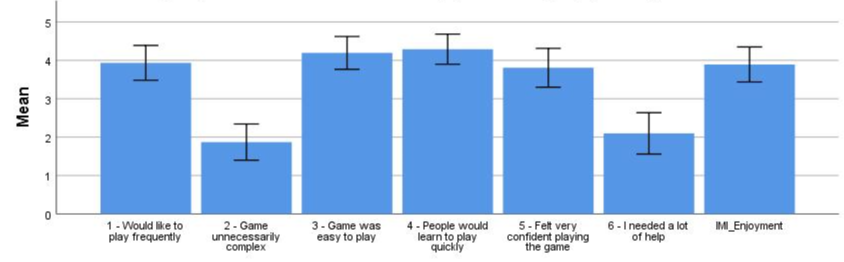
\includegraphics[scale = 0.35]{Mean.png}
	\caption{The mean results of the questionnaire, with a 95\% Confidence Interval. For questions 2 and 6, lower is better.}
	\label{fig:Evaluation1}
\end{figure}

\begin{figure}
	\centering
	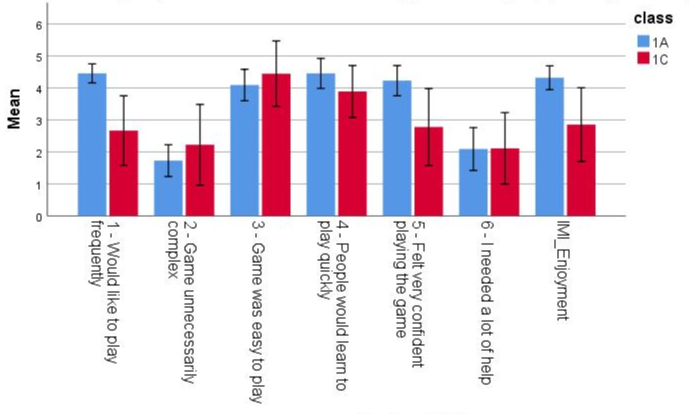
\includegraphics[scale = 0.4]{MeanPerClass.png}
	\caption{The mean results of the questionnaire per class, with a 95\% Confidence Interval. For questions 2 and 6, lower is better.}
	\label{fig:Evaluation2}
\end{figure}



